\documentclass[11pt]{article}
\usepackage[utf8]{inputenc}
\usepackage[T1, IL2]{fontenc}
\usepackage[czech]{babel}
\usepackage{url}
\usepackage{graphics}
\usepackage{amsmath}
\bibliographystyle{czechiso}
\begin{document}
\begin{titlepage}
\begin{center}
\textsc{\Huge Vysoké učení technické v~Brně\\ 
\vspace{\stretch{0.015}}
\huge Fakulta informačních technologií}\\
\vspace{\stretch{0.382}}
\LARGE Grafové algoritmy\\
\Huge 13. Hledání cyklů v orientovaném grafu\\
\vspace{\stretch{0.618}}
\Large \today \hfill Miroslav Paulík, Bc.\\ \hfill Igor Pavlů, Bc.
\end{center}
\end{titlepage}
\tableofcontents
\newpage
\section{Úvod}
Tato práce se zaměřuje na hledání cyklů v orientovaném grafu. Součástí je grafické uživatelské rozhraní, které je určeno pro snadnější zadávání grafů a vizuální demonstraci řešení. \\
	
\section{Analýza a řešení zadání}
K snadnému použití bylo zapotřebí sestavit grafické uživatelské rozhraní. Celá aplikace byla napsána v jazyce Python v2.7.6\cite{python} a grafické rozhraní pomocí grafické knihovny Tkinter\cite{tkinter}. Pro lepší týmovou spolupráci byl použit verzovací systém Git.\\ 
Součástí zadání bylo seznámení se s tzv. \textit{Johnsonovým algoritmem}\cite{jonshon}, který se vyznačuje časovou složitostí $O(|V|^2log|V| + |V||E|)$, kde $|V|$ je počet vrcholů a $|E|$ je počet hran gragu $G = (V, E)$. Díky problémům při implementaci vedoucím k fatálnímu selhání návrhu a časové tísni způsobené blížícím se termínem, bylo zapotřebí zvolit alternativní a méně efektivní řešení této problematiky.\\
Alternativní řešení spočívá v kombinaci algoritmu na vyhledávání silně souvyslích komponent\cite{gal} s využitím algoritmu DFS a následném prohledávání stavového prostoru. \\

\section{Ovládání}
Ovládání je intuitivní pomocí myši a to následovně:
\begin{enumerate}
	\item přidání uzlu -- dvojklik levého tlačítka myši
	\item přidání hrany -- kliknutí levým tlačítkem na uzel a tažení na cílový uzel
	\item přesun uzlu -- kliknutí pravým tlačítkem na uzel a tažení na požadované místo  
\end{enumerate}
Vlastní simulace se spouští pomocí tlačítka \textbf{Vyhledat cykly}, celá plocha se dá vymazat pomocí \textbf{Smazat graf}. Dále je možné aplikaci krokovat pomocí tlačítek \textbf{Předchozí cyklus} a \textbf{Následující cyklus}, dále je vložen ukázkový graf \textbf{Ukázka}.\\
Hrany odpovídající cyklům jsou zvýrazněny pomocí červené barvy.
Ukázka je na obrázku \ref{gui}
\begin{figure}[h!]
\begin{center}
\scalebox{1}{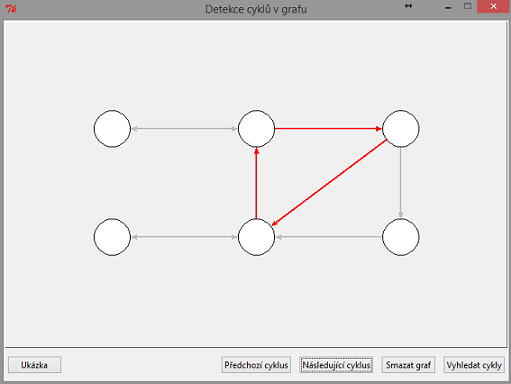
\includegraphics{gui.png}}
\caption{Grafické rozhraní}
\label{gui}
\end{center}
\end{figure} 
\section{Závěr}
Tato práce byla zaměřena na detekci cyklů v orientovaném grafu. Bohužel z technických důvodů nebyl použit doporučený Johnsonovým algoritmus, nicméně byla implementována alternativa detekce cyklů pomocí silně souvislých komponent a prohledávání stavového prostoru.\\ Tato aplikace nepřináší žádné speciální možnosti pro pokročilou analýzu grafů a slouží jen pro základní demonstrační účely. V případě dalšího vývoje by bylo třeba značně zapracovat na vnitřní implementaci algoritmů a jejich optimalizaci, stejně jako na grafickém rozhraní. Vhodné by bylo přidání možnosti načítání a ukládání dat například pomocí formátu \textit{GraphML}.
\newpage
\bibliography{literatura}
\end{document}